\documentclass[tikz,border=2pt]{standalone}
\usepackage{tikz}
\usetikzlibrary{calc}

\begin{document}
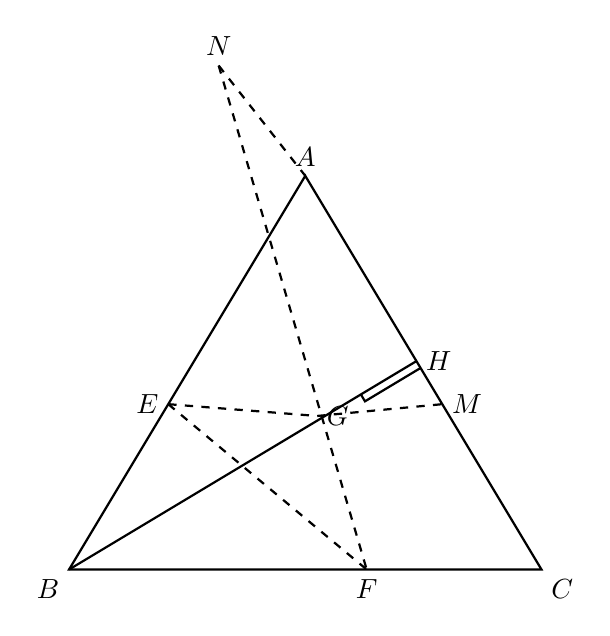
\begin{tikzpicture}[scale=1]

% Main triangle
\coordinate (B) at (0,0);
\coordinate (C) at (6,0);
\coordinate (A) at (3,5);

\draw[thick] (B)--(A)--(C)--cycle;

% Points on sides / interior
\coordinate (E) at ($(B)!0.42!(A)$);
\coordinate (F) at ($(B)!0.63!(C)$);
\coordinate (M) at ($(A)!0.58!(C)$);

% Dashed auxiliary points/lines from original figure
\coordinate (N) at ($(A)+(-1.1,1.4)$);
\coordinate (G) at (3.15,1.95);

\draw[dashed,thick] (N)--(F);
\draw[dashed,thick] (N)--(A);
\draw[dashed,thick] (E)--(G)--(M);
\draw[dashed,thick] (E)--(F);

% New edit: perpendicular from B to segment CM
\coordinate (H) at ($(C)!(B)!(M)$);
\draw[thick] (B)--(H);

% Right angle mark at H
\draw[thick] 
  ($(H)!0.16!(B)$) --
  ($($(H)!0.16!(B)$)+($(H)!0.16!(M)$)-(H)$) --
  ($(H)!0.16!(M)$);

% Labels
\node[below left] at (B) {$B$};
\node[below right] at (C) {$C$};
\node[above] at (A) {$A$};
\node[left] at (E) {$E$};
\node[below] at (F) {$F$};
\node[right] at (M) {$M$};
\node[above] at (N) {$N$};
\node[right] at (G) {$G$};
\node[right] at (H) {$H$};

\end{tikzpicture}
\end{document}
